\chapter[Continuous Deep Equilibrium Networks]{Continuous Deep Equilibrium Networks: Training Neural ODEs Faster by Integrating Them to Infinity}
\label{chapter:infinite_time_neural_odes}

Implicit layer methods, such as Neural ODEs and Deep Equilibrium models~\citep{chen2018neural, bai_deep_2019, ghaoui_implicit_2020}, have gained popularity due to their ability to automatically adapt model depth based on the ``complexity'' of new problems and inputs. The forward pass of these methods involves solving steady-state problems, convex optimization problems, differential equations, etc., all defined by neural networks, which can be expensive. However, training these more generalized models has empirically been shown to take significantly more time than traditional explicit models such as recurrent neural networks and transformers. \textit{Nothing within the problem's structure requires expensive training methods, so we asked, can we reformulate continuous implicit models so that this is not the case}?

\citet{grathwohl2018ffjord, dupont2019augmented, kelly2020learning, finlay2020train} have identified several problems with training implicit networks. These models grow in complexity as training progresses, and a single forward pass can take over 100 iterations~\citep{kelly2020learning} even for simple problems like MNIST. Deep Equilibrium Models~\citep{bai_deep_2019, bai_multiscale_2020} have better scaling in the backward pass but are still bottlenecked by slow steady-state convergence. \citet{bai2021stabilizing} quantified several convergence and stability problems with DEQs. They proposed a regularization technique by exploiting the ``implicitness" of DEQs to stabilize their training. \textit{We marry the idea of faster backward pass for DEQs and continuous modeling from Neural ODEs to create Infinite Time Neural ODEs which scale significantly better in the backward pass and drastically reduce the training time}. % However, such a regularization process is expensive as it requires higher-order automatic differentiation. Their results demonstrated faster prediction times at the expense of greatly increased training times. This leaves an open question as to whether such regularization could be imposed in a cheap or free enough manner to reduce the training cost.

Our main contributions include\footnote{Our code is publicly available at \url{https://github.com/SciML/DeepEquilibriumNetworks.jl}}:
%
\begin{enumerate}
    \item An improved DEQ architecture (Skip-DEQ) that uses an additional neural network to predict better initial conditions.

    \item A regularization scheme (Skip Regularized DEQ) incentivizes the DEQ to learn simpler dynamics and leads to faster training and prediction. Notably, this does not require nested automatic differentiation and thus is considerably less computationally expensive than other published techniques.

    \item A continuous formulation for DEQs as an infinite time neural ODE, which paradoxically accelerates the backward pass over standard neural ODEs by replacing the continuous adjoints with a simple linear system.

    \item We demonstrate the seamless combination of Continuous DEQs with Skip DEQs to create a drop-in replacement for Neural ODEs without incurring a high training cost.
\end{enumerate}
%

The contents of this chapter has appeared in the pre-print: Pal, A., Edelman, A. and Rackauckas, C., 2022. Continuous Deep Equilibrium Models: Training Neural ODEs Faster by Integrating Them to Infinity. arXiv preprint arXiv:2201.12240.~\citep{pal2022mixing}

\begin{figure}
    \centering
    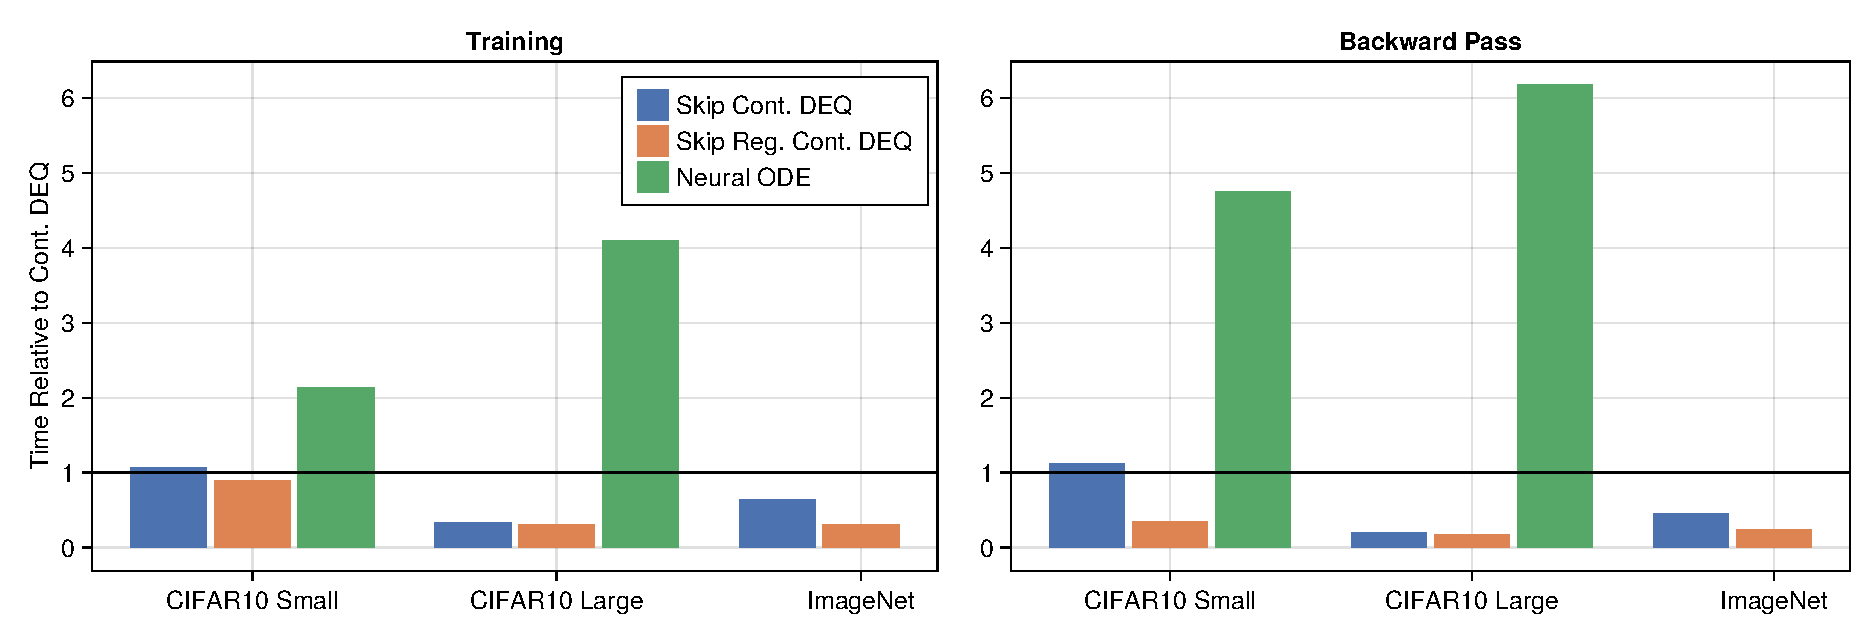
\includegraphics[width=\linewidth]{../figures/deep_equilibrium_models/summary_plot.pdf}
    \caption{\textbf{Relative Training and Backward Pass Timings against Continuous DEQs} \textit{(lower is better)}: In all scenarios, Neural ODEs take $\mathit{4.7} - \mathit{6.182 \times}$ more time in the backward pass compared to Vanilla Continuous DEQs. Whereas combining Skip (Reg.) with Continuous DEQs accelerates the backward pass by $\mathit{2.8} - \mathit{5.9 \times}$.}
    \label{fig:summary_plot}
\end{figure}

\section{Continuous Deep Equilibrium Networks}
\label{sec:continuous_deqs}

Deep Equilibrium Models have traditionally been formulated as steady-state problems for a discrete dynamical system. However, discrete dynamical systems come with a variety of shortcomings. Consider the following linear discrete dynamical system (See \Cref{fig:linear_discrete_dynamical_system}):
%
\begin{align}
    u_{n + 1}                   & = \alpha \cdot u_n         \\
    \texttt{ where } \|\alpha\| & < 1 \texttt{ and } u_0 = 1
\end{align}
%
This system converges to a steady state of $u_\infty = 0$. However, in many cases, this convergence can be relatively slow. If $\alpha = 0.9$, then after 10 steps, the value is $u_{10} = 0.35$ because a small amount only reduces each successive step. Thus convergence could only be accelerated by taking many steps together. Even further, if $\alpha = -0.9$, the value ping-pongs over the steady state $u_{1} = -0.9$, meaning that if we could take some fractional step $u_{\delta t}$ then it would be possible to approach the steady state much faster.

\begin{figure}[H]
    % Remove if space-constrained
    \centering
    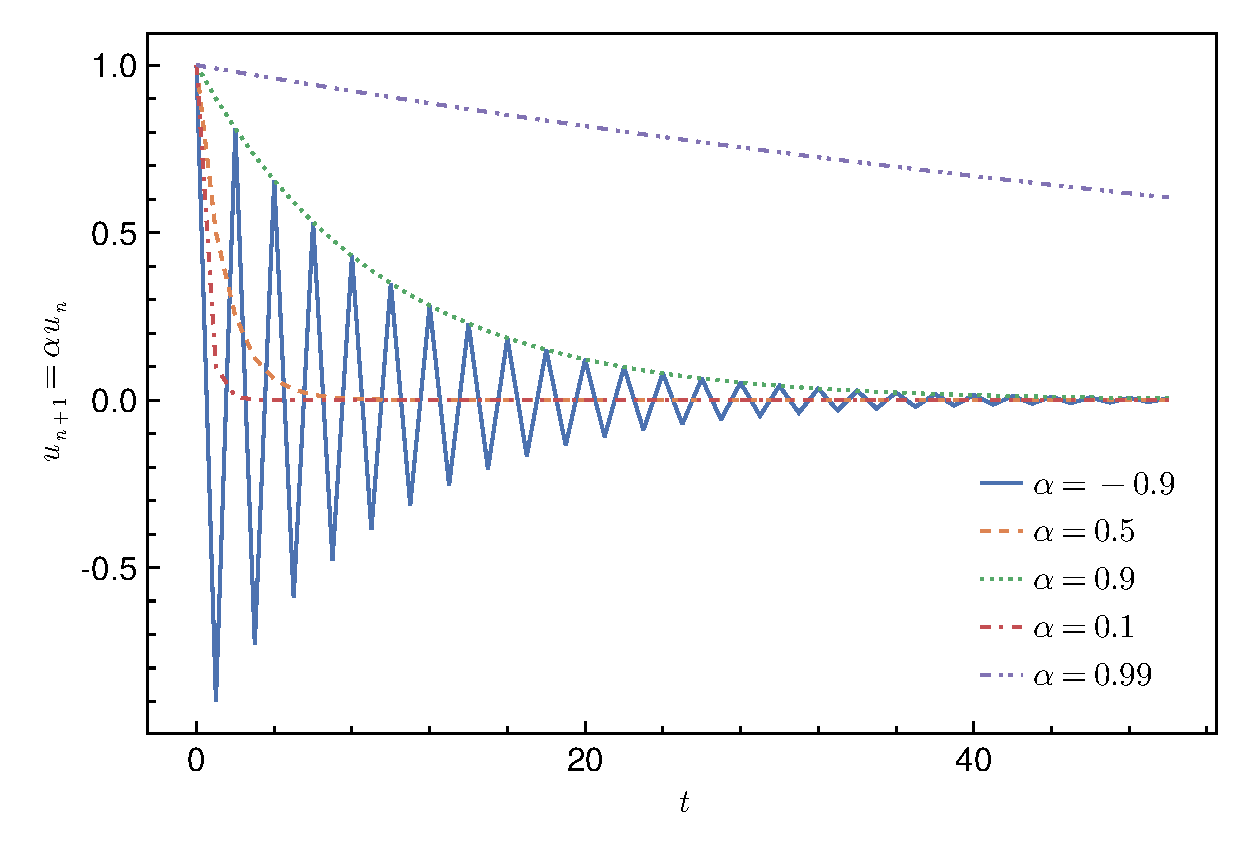
\includegraphics[width=0.8\linewidth]{../figures/deep_equilibrium_models/linear_discrete_dynamical_system.pdf}
    \caption{\textbf{Slow Convergence of Simple Linear Discrete Dynamical Systems}}
    \label{fig:linear_discrete_dynamical_system}
\end{figure}

\citet{rico1992discrete, bulsari1995neural} describe several other shortcomings of using discrete steady-state dynamics over continuous steady-state dynamics. These issues combined motivate changing from a discrete description of the system (the fixed point or Broyden's method approach) to a continuous description of the system that allows adaptivity to change the stepping behavior and accelerate convergence.

To this end, we propose an alternate formulation for DEQs by modeling a continuous dynamical system (Continuous DEQ) where the forward pass is represented by an ODE which is solved from $t_0 = 0$ to $t_1 = \infty$:
%
\begin{equation}
    \frac{dz}{dt} = \func{f_\theta}{z, x} - z
\end{equation}
%
where $f_\theta$ is an explicit neural network. Continuous DEQs leverage fast adaptive ODE solvers, which terminate automatically once the solution is close to a steady state, i.e., $\frac{dz^*}{dt} = 0$, which then satisfies $\func{f_\theta}{z^*, x} = z^*$ and is thus the solution to the same implicit system as before.

The Continuous DEQ can be considered an infinite-time neural ODE in this form. However, almost paradoxically, the infinite time version is cheaper to train than the finite time version as its solution is the solution to the nonlinear system, meaning the same implicit differentiation formula of the original DEQ holds for the derivative. This means that no backpropagation through the steps is required for the Continuous DEQ, and only a linear system must be solved. In \Cref{sec:infinite_time_neural_odes_experiments}, we empirically demonstrate that Continuous DEQs outperform Neural ODEs in terms of training time while achieving similar accuracies.

% Indeed, the robustness of the DEQ is even improved through this process because, in practice, the maximum iterations of the DEQ are bound~\citep{bai_deep_2019, bai_multiscale_2020, bai2021stabilizing}. DEQs often do not converge to a steady state due to this bound. In \Cref{sec:experiments}, we observe that for small-scale problems Skip~DEQs improve convergence to steady state  even where a DEQ fails due to its increased convergence speed. However, this behavior fades away once we move to the higher parameter count regime. When combining Skip~DEQs % This ability allows Skip DEQs to be trained with a more stable gradient signal since the adjoint equation assumes steady-state convergence during the forward pass.

\section{Skip Deep Equilibrium Networks}
\label{sec:skip_deqs}

\citet{bai_deep_2019, bai_multiscale_2020} set the initial condition $u_0 = 0$ while solving a DEQ. Assuming the existence of a steady state, the solvers will converge given enough iterations. However, each iteration is expensive, and a poor guess of the initial condition makes the convergence slower. To counteract these issues, we introduce an alternate architecture for DEQ (Skip~DEQ), where we use an explicit model $g_\phi$ to predict the initial condition for the steady-state problem $u_0 = g_\phi(x)$\footnote{We note that the concurrent work \citet{bai2021neural} introduced a similar formulation as a part of HyperDEQ}. We jointly optimize for $\left\{\theta, \phi\right\}$ by adding an auxiliary loss function:
%
\begin{equation}
    \mathcal{L}_{\texttt{skip}} = \lambda_{\texttt{skip}} \cdot \| f_\theta(z^*, x) - g_\phi(x) \|
\end{equation}
%
Intuitively, our explicit model $g_\phi$ better predicts a value closer to the steady-state (over the training iterations), and hence we need to perform fewer iterations during the forward pass. Given that its prediction is relatively free compared to the cost of the DEQ, this technique could decrease the cost of the DEQ by reducing the total number of iterations required. However, this prediction-correction approach still uses the result of the DEQ for its final predictions and thus should achieve robustness properties equal.

\section{Skip Regularized DEQ: Regularization Scheme without Extra Parameters}
\label{sec:skip_reg_deq}

One of the primary benefits of DEQs is the low memory footprint of these models. Introducing an explicit model $g_\phi$ increases the memory requirements for training. To alleviate this problem, we propose a regularization term to minimize the L1 distance between the first prediction of $f_\theta$ and the steady-state solution:
%
\begin{align}
    \mathcal{L}_{\texttt{skip\_reg}} = \lambda_{\texttt{skip}} \cdot \| f_\theta(z^*, x) - f_\theta(0, x) \|
\end{align}
%
This technique follows the same principle as the Skip DEQ where the DEQ's internal neural network is now treated as the prediction model. We hypothesize that this introduces an inductive bias in the model to learn simpler training dynamics.

\section{Experiments}
\label{sec:infinite_time_neural_odes_experiments}


In this section, we consider the effectiveness of our proposed methods -- Continuous DEQs and Skip DEQs -- on the training and prediction timings. We consider the following baselines:
%
\begin{enumerate}
    \item Discrete DEQs with L-Broyden Solver.
    \item Jacobian Regularization of DEQs.\footnote{We note that due to limitations of our Automatic Differentiation system, we cannot perform Jacobian Regularization for Convolutional Models. However, our preliminary analysis suggests that the Skip DEQ and Continuous DEQ approaches are fully composable with Jacobian Regularization and provide better performance compared to using only Jacobian Regularization (See \Cref{tab:mnist_dense_summary}).}
    \item Multi-Scale Neural ODEs with Input Injection: A modified Continuous Multiscale DEQ without the steady state convergence constaint.
\end{enumerate}
%
Our primary metrics are classification accuracy, the number of function evaluations (NFEs), total training time, time for the backward pass, and prediction time per batch. We showcase the performance of our methods on -- MNIST~\citep{lecun1998gradient}, CIFAR-10~\citep{krizhevsky2009learning}, SVHN~\citep{netzer2011reading}, \& ImageNet~\citep{deng2009imagenet}. We use perform our experiments in Julia~\citep{Julia-2017} using Lux.jl~\citep{pal2022lux} and DifferentialEquations.jl~\citep{DifferentialEquations.jl-2017, rackauckas2018comparison, rackauckas2020universal}.

\subsection{MNIST Image Classification}
\label{subsec:infinite_time_neural_odes_mnist_image_classification}

\begin{table}[t]
    \centering
    \adjustbox{max width=\linewidth}{
        \centering
        \begin{tabular}{lcccccc}
            \toprule
            \thead{Model} & \thead{Jacobian Reg.} & \thead{\# of Params} & \thead{Test Accuracy (\%)} & \thead{Testing NFE}        & \thead{Training Time (min)} & \thead{Prediction Time (s / batch)} \\
            \midrule
            Vanilla DEQ   & \crossmark            & 138K                 & \sdval{97.926}{0.107}      & \sdval{18.345}{0.732}      & \sdval{5.197}{1.106}        & \sdval{0.038}{0.009}                \\
                          & \tickmark             &                      & \sdval{98.123}{0.025}      & \sdval{\hp{0}5.034}{0.059} & \sdval{7.321}{0.454}        & \sdval{0.011}{0.005}                \\
            \addlinespace
            Skip DEQ      & \crossmark            & 151K                 & \sdval{97.759}{0.080}      & \sdval{\hp{0}4.001}{0.001} & \sdval{1.711}{0.202}        & \sdval{0.010}{0.001}                \\
                          & \tickmark             &                      & \sdval{97.749}{0.141}      & \sdval{\hp{0}4.001}{0.000} & \sdval{6.019}{0.234}        & \sdval{0.012}{0.001}                \\
            \addlinespace
            Skip Reg. DEQ & \crossmark            & 138K                 & \sdval{97.973}{0.134}      & \sdval{\hp{0}4.001}{0.000} & \sdval{1.295}{0.222}        & \sdval{0.010}{0.001}                \\
                          & \tickmark             &                      & \sdval{98.016}{0.049}      & \sdval{\hp{0}4.001}{0.000} & \sdval{5.128}{0.241}        & \sdval{0.012}{0.000}                \\
            \bottomrule
        \end{tabular}
    }
    \caption{\textbf{MNIST Classification with Fully Connected Layers}: Skip Reg. Continuous DEQ without Jacobian Regularization takes \textit{$\mathit{4\times}$ less training time} and \textit{speeds up prediction time by $4\times$} compared to Continuous DEQ. Continuous DEQ with Jacobian Regularization has a similar prediction time but takes \textit{$\mathit{6\times}$ more training time} than Skip Reg. Continuous DEQ. Using Skip variants \textit{speeds up training by $\mathit{1.42\times - 4\times}$}.}
    \label{tab:mnist_dense_summary}
\end{table}

\textbf{Training Details:} Following \citet{kelly2020learning}, our Fully Connected Model consists of 3 layers -- a downsampling layer $\mathbb{R}^{784} \mapsto \mathbb{R}^{128}$, continuous DEQ layer $f_\theta: \mathbb{R}^{128} \mapsto \mathbb{R}^{128}$, and a linear classifier $\mathbb{R}^{128} \mapsto \mathbb{R}^{10}$.

For regularization, we use $\lambda_{\texttt{skip}} = 0.01$ and train the models for $25$ epochs with a batch size of $32$. We use Tsit5~\citep{tsitouras2011runge} with a relative tolerance for convergence of $0.005$. For optimization, we use Adam~\citep{kingma2014adam} with a constant learning rate of $0.001$.

\textbf{Baselines:} We use continuous DEQ and continuous DEQ with Jacobian Stabilization as our baselines. We additionally compose Skip DEQs with Jacobian Stabilization in our benchmarks. For all experiments, we keep $\lambda_{\texttt{jac}} = 1.0$.

\textbf{Results:} We summarize our results in \Cref{tab:mnist_dense_summary}. Without Jacobian Stabilization, Skip Reg. Continuous DEQ has the highest testing accuracy of $\mathit{97.973\%}$ and has the \textit{lowest training and prediction timings overall}. Using Jacobian Regularization, DEQ outperforms Skip~DEQ models by $\mathit{< 0.4\%}$, however, jacobian regularization increases training time by $\mathit{1.4 - 4}\times$. Skip~DEQ models can obtain the lowest prediction time per batch of $\mathit{\sim0.01s}$.

\subsection{CIFAR10 Image Classification}
\label{subsec:infinite_time_neural_odes_cifar10_image_classification}

\begin{table}[t]
    \centering
    \adjustbox{max width=\linewidth}{
        \centering
        \begin{tabular}{lcccccc}
            \toprule
            \thead{Model} & \thead{Continuous} & \thead{\# of Params} & \thead{Test Accuracy (\%)} & \thead{Training Time                                               \\ (s / batch)} & \thead{Backward Pass\\ (s / batch)} & \thead{Prediction Time\\ (s / batch)}\\
            \midrule
            Vanilla DEQ   & \crossmark         & 163546               & \sdval{81.233}{0.097}      & \sdval{0.651}{0.009} & \sdval{0.075}{0.001} & \sdval{0.282}{0.005} \\
                          & \tickmark          &                      & \sdval{80.807}{0.631}      & \sdval{0.753}{0.017} & \sdval{0.261}{0.010} & \sdval{0.136}{0.010} \\
            \addlinespace
            Skip DEQ      & \crossmark         & 200122               & \sdval{82.013}{0.306}      & \sdval{0.717}{0.022} & \sdval{0.115}{0.004} & \sdval{0.274}{0.005} \\
                          & \tickmark          &                      & \sdval{80.807}{0.230}      & \sdval{0.806}{0.010} & \sdval{0.293}{0.004} & \sdval{0.154}{0.002} \\
            \addlinespace
            Skip Reg. DEQ & \crossmark         & 163546               & \sdval{81.170}{0.356}      & \sdval{0.709}{0.005} & \sdval{0.114}{0.002} & \sdval{0.283}{0.007} \\
                          & \tickmark          &                      & \sdval{82.513}{0.177}      & \sdval{0.679}{0.015} & \sdval{0.143}{0.017} & \sdval{0.154}{0.003} \\
            \addlinespace
            Neural ODE    & \tickmark          & 163546               & \sdval{83.543}{0.393}      & \sdval{1.608}{0.026} & \sdval{1.240}{0.021} & \sdval{0.207}{0.006} \\
            \bottomrule
        \end{tabular}
    }
    \caption{\textbf{CIFAR10 Classification with Small Neural Network}: Skip Reg. Continuous DEQ achieves the \textit{highest test accuracy among DEQs}. Continuous DEQs are faster than Neural ODEs during training by a factor of $\mathit{2\times - 2.36\times}$, with a speedup of $\mathit{4.2\times - 8.67\times}$ in the backward pass. We also observe a prediction speed-up for Continuous DEQs of $\mathit{1.77\times - 2.07\times}$ against Discrete DEQs and $\mathit{1.34\times - 1.52\times}$ against Neural ODE.}
    \label{tab:cifar10_tiny_summary}
\end{table}

\begin{figure}[t]
    \centering
    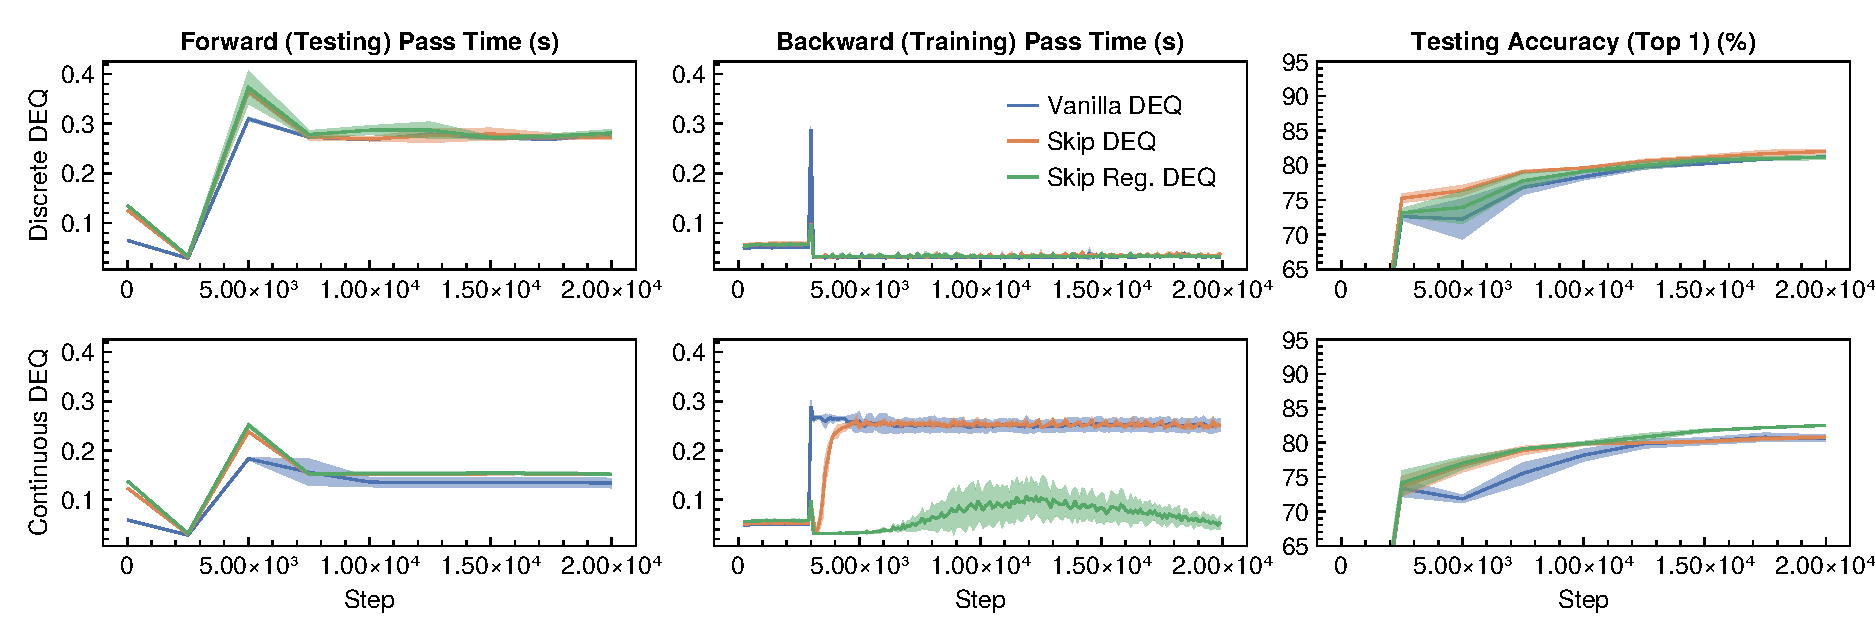
\includegraphics[width=\linewidth]{../figures/deep_equilibrium_models/cifar10_tiny.pdf}
    \caption{\textbf{CIFAR10 Classification with Small Neural Network}}
    \label{fig:cifar10_tiny}
\end{figure}


For all the baselines in this section, Vanilla DEQ is trained with the same training hyperparameters as the corresponding Skip DEQs (taken from \citet{bai_multiscale_2020}). Multiscale Neural ODE with Input Injection is trained with the same hyperparameters as the corresponding Continuous DEQs.

\subsubsection{Architecture with ~200K parameters}

% \input{tables/imagenet.tex}

\textbf{Training Details:} Our Multiscale DEQ architecture is the same as MDEQ-small architecture used in \citet{bai_multiscale_2020}. For the explicit network in Skip~DEQ, we use the residual block and downsampling blocks from \citet{bai_multiscale_2020} which account for the additional 58K trainable parameters.

We use a fixed regularization weight of $\lambda_{\texttt{skip}} = 0.01$ and the models are trained for 20000 steps. We use a batch size of $128$. For continuous models, we use VCAB3~\citep{wanner1996solving} with a relative tolerance for convergence of $0.05$. We use AdamW~\citep{loshchilov2017decoupled} optimizer with a cosine scheduling on the learning rate -- starting from $10^{-3}$ and terminating at $10^{-6}$ -- and a weight decay of $2.5 \times 10^{-6}$.

\textbf{Results:} We summarize our results in \Cref{tab:cifar10_tiny_summary} and \Cref{fig:cifar10_tiny}. Continuous DEQs are faster than Neural ODEs during training by a factor of $\mathit{2\times - 2.36\times}$, with a speedup of $\mathit{4.2\times - 8.67\times}$ in the backward pass.

\begin{table}[t]
    \centering
    \adjustbox{max width=\linewidth}{
        \centering
        \begin{tabular}{lcccccc}
            \toprule
            \thead{Model} & \thead{Continuous} & \thead{\# of Params} & \thead{Test Accuracy (\%)} & \thead{Training Time                                               \\ (s / batch)} & \thead{Backward Pass\\ (s / batch)} & \thead{Prediction Time\\ (s / batch)}\\
            \midrule
            Vanilla DEQ   & \crossmark         & 10.63M               & \sdval{88.913}{0.287}      & \sdval{0.625}{0.165} & \sdval{0.111}{0.021} & \sdval{0.414}{0.222} \\
                          & \tickmark          &                      & \sdval{89.367}{0.832}      & \sdval{1.284}{0.011} & \sdval{0.739}{0.003} & \sdval{0.606}{0.010} \\
            \addlinespace
            Skip DEQ      & \crossmark         & 11.19M               & \sdval{88.783}{0.178}      & \sdval{0.588}{0.042} & \sdval{0.112}{0.006} & \sdval{0.314}{0.017} \\
                          & \tickmark          &                      & \sdval{89.600}{0.947}      & \sdval{0.697}{0.012} & \sdval{0.150}{0.013} & \sdval{0.625}{0.004} \\
            \addlinespace
            Skip Reg. DEQ & \crossmark         & 10.63M               & \sdval{88.773}{0.115}      & \sdval{0.613}{0.048} & \sdval{0.109}{0.008} & \sdval{0.268}{0.031} \\
                          & \tickmark          &                      & \sdval{90.107}{0.837}      & \sdval{0.660}{0.019} & \sdval{0.125}{0.003} & \sdval{0.634}{0.019} \\
            \addlinespace
            Neural ODE    & \tickmark          & 10.63M               & \sdval{89.047}{0.116}      & \sdval{5.267}{0.078} & \sdval{4.569}{0.077} & \sdval{0.573}{0.010} \\
            \bottomrule
        \end{tabular}
    }
    \caption{\textbf{CIFAR10 Classification with Large Neural Network}: Skip Reg. Continuous DEQ achieves the \textit{highest test accuracy}. Continuous DEQs are faster than Neural ODEs during training by a factor of \timeschange{4.1}{7.98}, with a speedup of \timeschange{6.18}{36.552} in the backward pass. However, we observe a prediction slowdown for Continuous DEQs of \timeschange{1.4}{2.36} against Discrete DEQs and \timeschange{0.90}{0.95} against Neural ODE.}
    \label{tab:cifar10_large_summary}
\end{table}

\begin{figure}[t]
    \centering
    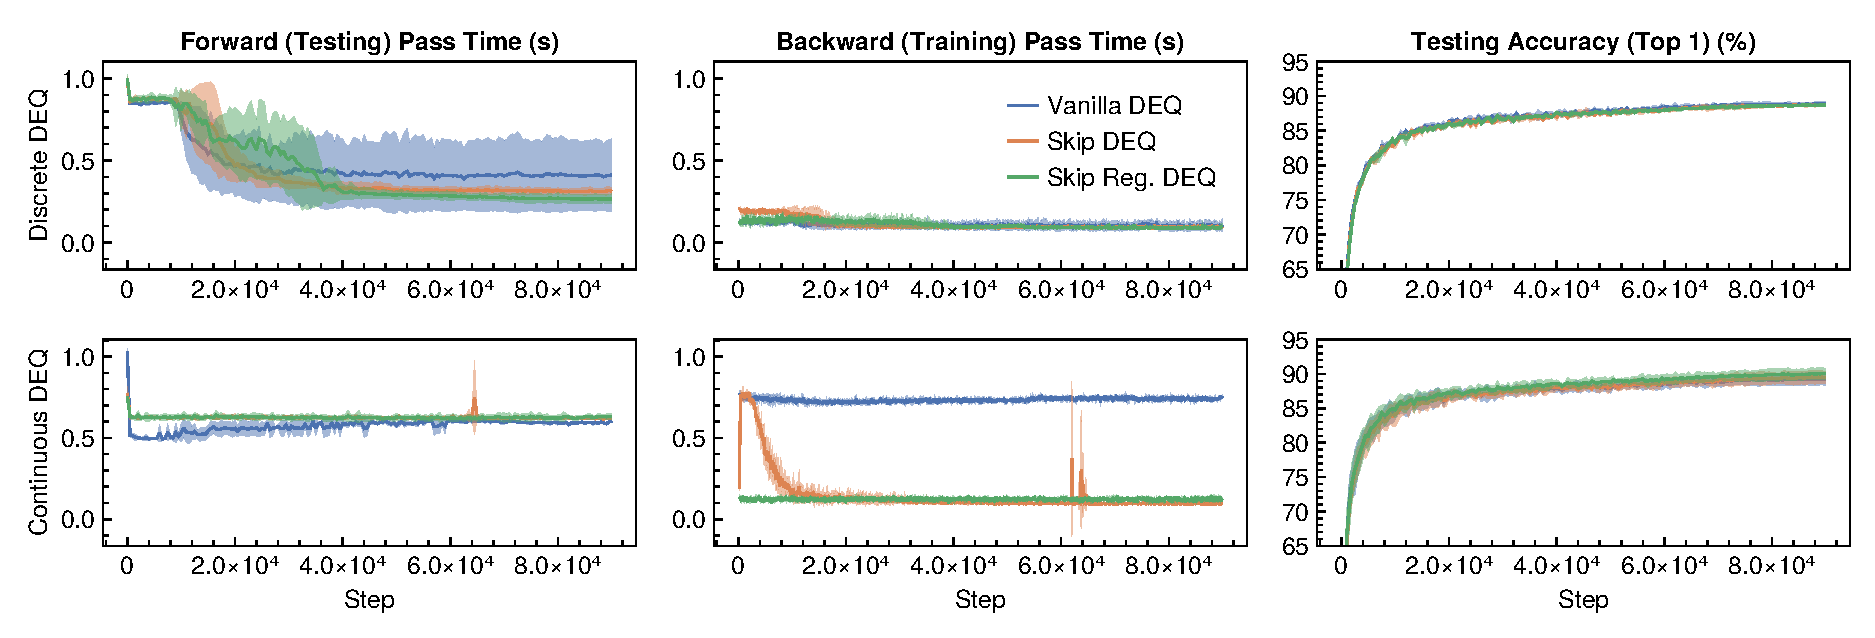
\includegraphics[width=\linewidth]{../figures/deep_equilibrium_models/cifar10_large}
    \caption{\textbf{CIFAR10 Classification with Large Neural Network}}
    \label{fig:cifar10_large}
\end{figure}

\subsubsection{Architecture with 11M parameters}

\textbf{Training Details:} Our Multiscale DEQ architecture is the same as MDEQ-large architecture used in \citet{bai_multiscale_2020}. For the explicit network in Skip~DEQ, we use the residual block and downsampling blocks from \citet{bai_multiscale_2020} which account for the additional 58K trainable parameters.

We use a fixed regularization weight of $\lambda_{\texttt{skip}} = 0.01$ and the models are trained for 90000 steps. We use a batch size of $128$. For continuous models, we use VCAB3~\citep{wanner1996solving} with a relative tolerance for convergence of $0.05$. We use Adam~\citep{kingma2014adam} optimizer with a cosine scheduling on the learning rate -- starting from $10^{-3}$ and terminating at $10^{-6}$.

\textbf{Results:} We summarize our results in \Cref{tab:cifar10_large_summary} and \Cref{fig:cifar10_large}. Continuous DEQs are faster than Neural ODEs during training by a factor of \timeschange{4.1}{7.98}, with a speedup of \timeschange{6.18}{36.552} in the backward pass.


\begin{figure}[t]
    \centering
    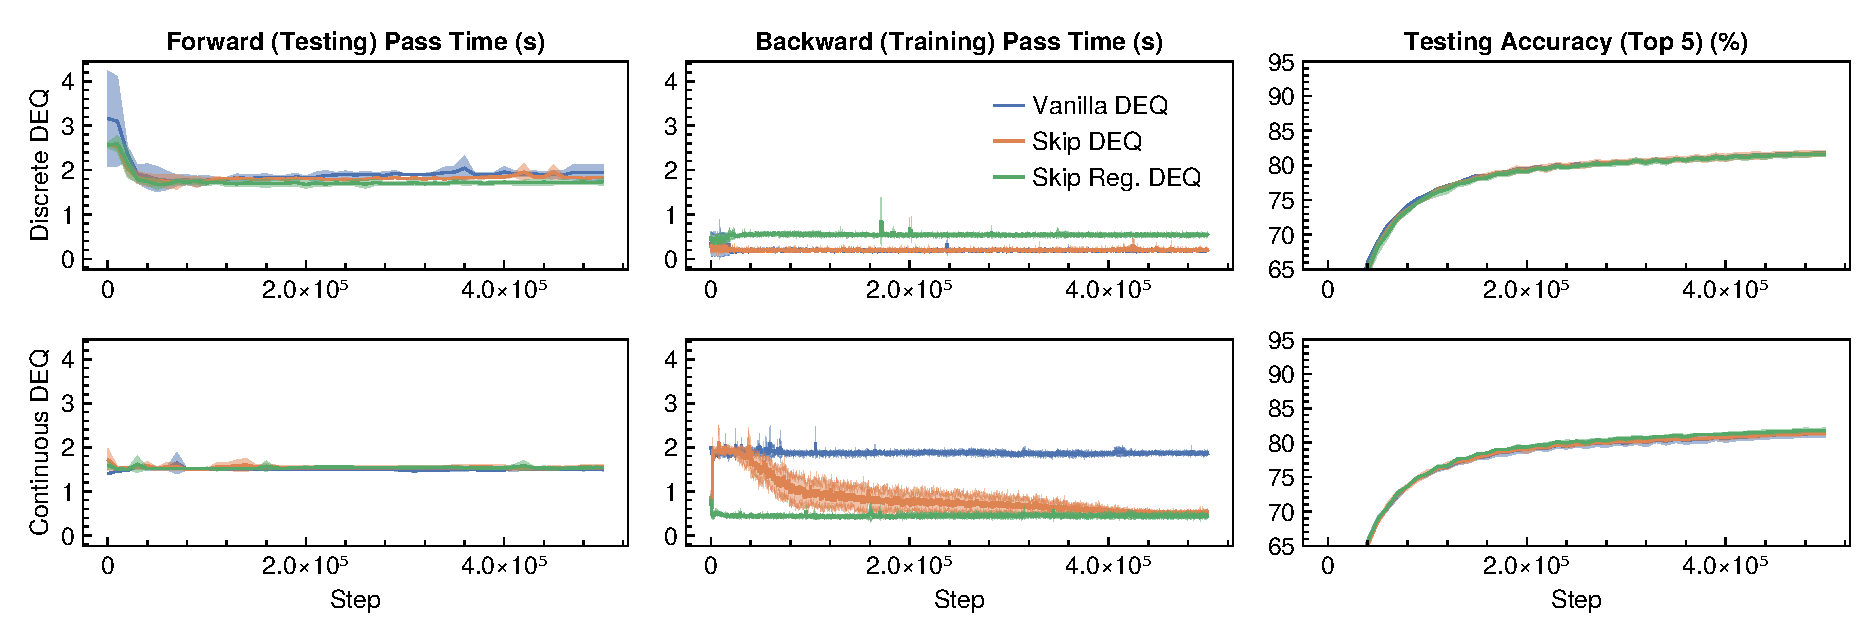
\includegraphics[width=\linewidth]{../figures/deep_equilibrium_models/imagenet_small}
    \caption{\textbf{ImageNet Classification}}
    \label{fig:imagenet_small}
\end{figure}
\subsection{ImageNet Image Classification}
\label{subsec:infinite_time_neural_odes_imagenet_image_classification}

\begin{table}[t]
    \centering
    \adjustbox{max width=\linewidth}{
        \centering
        \begin{tabular}{lcccccc}
            \toprule
            \thead{Model} & \thead{Continuous} & \thead{\# of Params} & \thead{Test Accuracy                                                                       \\ (Top 5) (\%)} & \thead{Training Time\\ (s / batch)} & \thead{Backward Pass\\ (s / batch)} & \thead{Prediction Time\\ (s / batch)}\\
            \midrule
            Vanilla DEQ   & \crossmark         & 17.91M               & \sdval{81.809}{0.115} & \sdval{2.057}{0.138} & \sdval{0.195}{0.007} & \sdval{1.963}{0.189} \\
                          & \tickmark          &                      & \sdval{81.329}{0.516} & \sdval{3.131}{0.027} & \sdval{1.873}{0.015} & \sdval{1.506}{0.027} \\
            \addlinespace
            Skip DEQ      & \crossmark         & 18.47M               & \sdval{81.717}{0.452} & \sdval{1.956}{0.012} & \sdval{0.194}{0.001} & \sdval{1.843}{0.025} \\
                          & \tickmark          &                      & \sdval{81.334}{0.322} & \sdval{2.016}{0.129} & \sdval{0.845}{0.127} & \sdval{1.575}{0.053} \\
            \addlinespace
            Skip Reg. DEQ & \crossmark         & 17.91M               & \sdval{81.611}{0.369} & \sdval{1.996}{0.035} & \sdval{0.539}{0.023} & \sdval{1.752}{0.093} \\
                          & \tickmark          &                      & \sdval{81.813}{0.350} & \sdval{1.607}{0.044} & \sdval{0.444}{0.026} & \sdval{1.560}{0.021} \\
            % \addlinespace
            % Neural ODE & \tickmark & 17.91M & & & &\\
            \bottomrule
        \end{tabular}
    }
    \caption{\textbf{ImageNet Classification}: All the variants attain comparable evaluation accuracies. Skip (Reg.) accelerates the training of Continuous DEQ by $\mathit{1.57\times - 1.96\times}$, with a reduction of $\mathit{2.2\times - 4.2\times}$ in the backward pass timings. However, we observe a marginal increase of $\mathit{4\%}$ in prediction timings for Skip (Reg.) Continuous DEQ compared against Continuous DEQ. For Discrete DEQs, Skip (Reg.) variants reduce the prediction timings by $\mathit{6.5\% - 12\%}$.}
    \label{tab:imagenet_summary}
\end{table}

\textbf{Training Details:} Our Multiscale DEQ architecture is the same as MDEQ-small architecture used in \citet{bai_multiscale_2020}. For the explicit network in Skip~DEQ, we use the residual block and downsampling blocks from \citet{bai_multiscale_2020} which account for the additional 58K trainable parameters.

We use a fixed regularization weight of $\lambda_{\texttt{skip}} = 0.01$, and the models are trained for 500000 steps. We use a batch size of $64$. For continuous models, we use VCAB3~\citep{wanner1996solving} with a relative tolerance for convergence of $0.05$. We use SGD with a momentum of $0.9$ and weight decay of $10^{-6}$. We use a step LR scheduling reducing the learning rate from $0.05$ by a multiplicative factor of $0.1$ at steps $100000$, $150000$, and $250000$.

\textbf{Baselines:} Vanilla DEQ is trained with the same training hyperparameters as the corresponding Skip DEQs (taken from \citep{bai_multiscale_2020})\footnote{When training MultiScale Neural ODE with the same configuration as Continuous DEQ, we observed a $\mathit{8\times}$ slower backward pass which made the training of the baseline infeasible.}.

\textbf{Results:} We summarize our results in \Cref{tab:imagenet_summary} and \Cref{fig:imagenet_small}. Skip (Reg.) variants accelerate the training of Continuous DEQ by $\mathit{1.57\times - 1.96\times}$, with a reduction of $\mathit{2.2\times - 4.2\times}$ in the backward pass timings.


\section{Discussion}
\label{sec:infinite_time_neural_odes_conclusion}

We have empirically shown the effectiveness of Continuous~DEQs as a faster alternative for Neural ODEs. Consistent with the ablation studies in \citet{bai2021neural}, we see that Skip DEQ in itself doesn't significantly improve the prediction or training timings for Discrete DEQs. Skip Reg. DEQ does, however, speeds up the inference for larger Discrete DEQs. However, combining Skip DEQ and Skip Reg. DEQ with Continuous DEQs, enable a speedup in backward pass by over $\mathit{2.8} - \mathit{5.9 \times}$. We hypothesize that this improvement is due to reduction in the condition number, which results in faster convergence of GMRES in the backward pass, however, acertaining this would require furthur investigation. We have demonstrated that our improvements to DEQs and Neural ODEs enable the drop-in replacement of Skip Continuous DEQs in any classical deep learning problem where continuous implicit models were previously employed.

\subsection{Limitations}
\label{sec:infinite_time_neural_odes_limitations}

We observe the following limitations for our proposed methods:
%
\begin{itemize}
    \item Reformulating a Neural ODE as a Continuous DEQ is valid, when the actual dynamics of the system doesn't matter. This holds true for all applications of Neural ODEs to classical Deep Learning problems.

    \item Continuous DEQs are slower than their Discrete counterparts for larger models (without any significant improvement to accuracy), hence the authors recommend their usage only for cases where a continuous model is truly needed.
\end{itemize}
%